\documentclass{standalone}
\usepackage{tikz}
\usepackage{amsmath}

\begin{document}

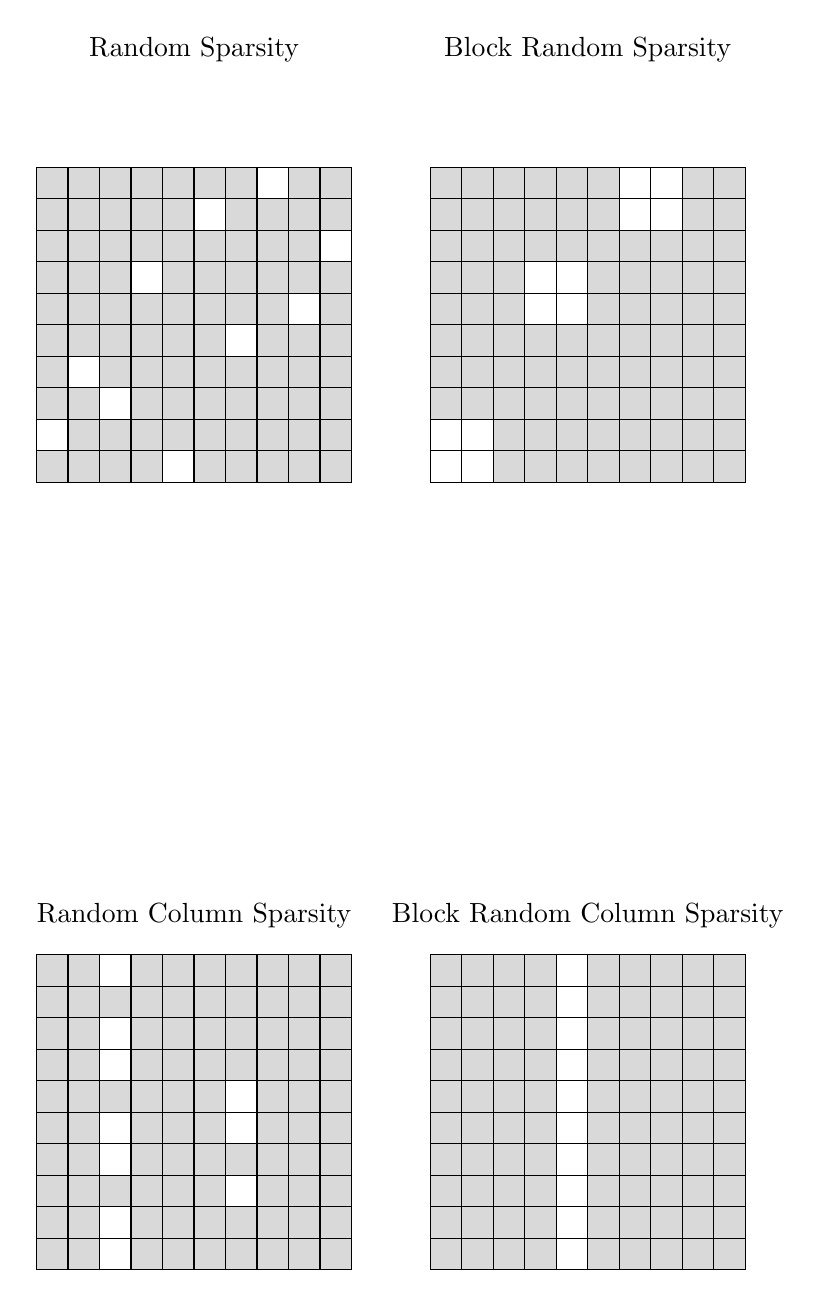
\begin{tikzpicture}
    \def\squaresize{0.4}
    \def\gridsize{10}

    % Random Sparsity
    \node at (2, 5.5) {Random Sparsity};
    \foreach \x in {0,...,9} {
        \foreach \y in {0,...,9} {
            \filldraw[fill=gray!30, draw=black] (\x*\squaresize, \y*\squaresize) rectangle ++(\squaresize, \squaresize);
        }
    }
    \foreach \x/\y in {0/1, 1/3, 2/2, 3/6, 4/0, 5/8, 6/4, 7/9, 8/5, 9/7} {
        \filldraw[fill=white, draw=black] (\x*\squaresize, \y*\squaresize) rectangle ++(\squaresize, \squaresize);
    }

    % Block Random Sparsity
    \node at (7, 5.5) {Block Random Sparsity};
    \foreach \x in {0,...,9} {
        \foreach \y in {0,...,9} {
            \filldraw[fill=gray!30, draw=black] (\x*\squaresize + 5, \y*\squaresize) rectangle ++(\squaresize, \squaresize);
        }
    }
    \foreach \x/\y in {0/0, 0/1, 1/0, 1/1, 3/5, 3/6, 4/5, 4/6, 6/8, 6/9, 7/8, 7/9} {
        \filldraw[fill=white, draw=black] (\x*\squaresize + 5, \y*\squaresize) rectangle ++(\squaresize, \squaresize);
    }

    % Random Column Sparsity
    \node at (2, -5.5) {Random Column Sparsity};
    \foreach \x in {0,...,9} {
        \foreach \y in {0,...,9} {
            \filldraw[fill=gray!30, draw=black] (\x*\squaresize, \y*\squaresize - 10) rectangle ++(\squaresize, \squaresize);
        }
    }
    \foreach \x/\y in {2/0, 2/1, 2/3, 2/4, 2/6, 2/7, 2/9, 6/2, 6/4, 6/5} {
        \filldraw[fill=white, draw=black] (\x*\squaresize, \y*\squaresize - 10) rectangle ++(\squaresize, \squaresize);
    }

    % Block Random Column Sparsity
    \node at (7, -5.5) {Block Random Column Sparsity};
    \foreach \x in {0,...,9} {
        \foreach \y in {0,...,9} {
            \filldraw[fill=gray!30, draw=black] (\x*\squaresize + 5, \y*\squaresize - 10) rectangle ++(\squaresize, \squaresize);
        }
    }
    \foreach \x/\y in {4/0, 4/1, 4/2, 4/3, 4/4, 4/5, 4/6, 4/7, 4/8, 4/9} {
        \filldraw[fill=white, draw=black] (\x*\squaresize + 5, \y*\squaresize - 10) rectangle ++(\squaresize, \squaresize);
    }

\end{tikzpicture}

\end{document}